\documentclass[12pt,a4paper,titlepage]{article}
\usepackage[utf8]{inputenc}
\usepackage[T1]{fontenc}
\usepackage[french]{babel}
\usepackage{graphicx}
\usepackage{amsthm}
\usepackage{amsmath, amsfonts}
\usepackage{amssymb}
\usepackage{mathrsfs}
\usepackage{color}
\usepackage{colortbl}
\usepackage{url}
\usepackage{color}
\usepackage{listings}

\definecolor{mygreen}{RGB}{28,172,0} % color values Red, Green, Blue
\definecolor{mylilas}{RGB}{170,55,241}

\lstset{
language=R,
basicstyle=\scriptsize\ttfamily,
commentstyle=\ttfamily\color{green},
numbers=left,
numberstyle=\ttfamily\color{black}\footnotesize,
stepnumber=1,
numbersep=5pt,
backgroundcolor=\color{white},
showspaces=false,
showstringspaces=false,
showtabs=false,
frame=single,
tabsize=2,
captionpos=b,
breaklines=true,
breakatwhitespace=false,
keywordstyle=\color{blue},
stringstyle=\color{magenta},
literate=
  {á}{{\'a}}1 {é}{{\'e}}1 {í}{{\'i}}1 {ó}{{\'o}}1 {ú}{{\'u}}1
  {Á}{{\'A}}1 {É}{{\'E}}1 {Í}{{\'I}}1 {Ó}{{\'O}}1 {Ú}{{\'U}}1
  {à}{{\`a}}1 {è}{{\`e}}1 {ì}{{\`i}}1 {ò}{{\`o}}1 {ù}{{\`u}}1
  {À}{{\`A}}1 {È}{{\'E}}1 {Ì}{{\`I}}1 {Ò}{{\`O}}1 {Ù}{{\`U}}1
  {ä}{{\"a}}1 {ë}{{\"e}}1 {ï}{{\"i}}1 {ö}{{\"o}}1 {ü}{{\"u}}1
  {Ä}{{\"A}}1 {Ë}{{\"E}}1 {Ï}{{\"I}}1 {Ö}{{\"O}}1 {Ü}{{\"U}}1
  {â}{{\^a}}1 {ê}{{\^e}}1 {î}{{\^i}}1 {ô}{{\^o}}1 {û}{{\^u}}1
  {Â}{{\^A}}1 {Ê}{{\^E}}1 {Î}{{\^I}}1 {Ô}{{\^O}}1 {Û}{{\^U}}1
  {œ}{{\oe}}1 {Œ}{{\OE}}1 {æ}{{\ae}}1 {Æ}{{\AE}}1 {ß}{{\ss}}1
  {ű}{{\H{u}}}1 {Ű}{{\H{U}}}1 {ő}{{\H{o}}}1 {Ő}{{\H{O}}}1
  {ç}{{\c c}}1 {Ç}{{\c C}}1 {ø}{{\o}}1 {å}{{\r a}}1 {Å}{{\r A}}1
  {€}{{\EUR}}1 {£}{{\pounds}}1
}


\lstset{language=Matlab,%
    %basicstyle=\color{red},
    breaklines=true,%
    morekeywords={matlab2tikz},
    keywordstyle=\color{blue},%
    morekeywords=[2]{1}, keywordstyle=[2]{\color{black}},
    identifierstyle=\color{black},%
    stringstyle=\color{mylilas},
    commentstyle=\color{mygreen},%
    showstringspaces=false,%without this there will be a symbol in the places where there is a space
    numbers=left,%
    numberstyle={\tiny \color{black}},% size of the numbers
    numbersep=9pt, % this defines how far the numbers are from the text
    emph=[1]{for,end,break},emphstyle=[1]\color{red}, %some words to emphasise
    %emph=[2]{word1,word2}, emphstyle=[2]{style},    
}

\title{OS13 : Test d'estimation et loi extrême des lois de Cauchy et géométrique}
\author{\textsc{Adrien WARTELLE} \\ \textsc{TRAN Quoc Nhat Han}}
\date{\today}

\begin{document}

\maketitle 
\renewcommand{\contentsname}{Sommaire}
\tableofcontents

\newpage

\section{Loi géométrique}

La loi géomètrique est une loi discrète de distribution utilisé
dans le cadre d'un enchainement (non fini) d'épreuves de Bernouilli. Soit
X une varaible aléatoire suivant cette loi, on a:
\[P(X=k) = (1-p)^(k-1)p\ k\in\mathbb{N}_{+}\]
La variable X est le numéro de la première épreuve où l'on obtient un succès
qui a une probabilité p. Ainsi, p est le seul paramètre de loi (à estimer).
La fonction de répartition $F(k) = P(X\leq{}k)\ k\in\mathbb{N}_{+}$ est:
\[F(k)=1-(1-p)^{k}\]
\begin{proof}
On peut remarquer que:
\[P(X=k)=(1-p)^{k-1}(1-(1-p))=(1-p)^{k-1}-(1-p)^{k}\]
Donc :
\[F(k)=\sum\limits_{l=1}^{k}P(X=l)=\sum\limits_{l=1}^{k}((1-p)^{l-1}-(1-p)^{l})\]
\[F(k)=\sum\limits_{l=0}^{k-1}(1-p)^{l}-\sum\limits_{l=1}^{k}(1-p)^{l}\]
Soit $q=1-p$, on a :
\[F(k)=\sum\limits_{l=0}^{k-1}q^{l}-\sum\limits_{l=1}^{k}q^{l}\]
\[F(k)=\frac{1-p^k}{1-q}-(\frac{1-q^{k+1}}{1-q}-1)\]
\[F(k)=\frac{1-q^k-1+q^{k+1}+1-q}{1-q}\]
\[F(k)=\frac{1-q+q^{k+1}-q^k}{1-q}\]
\[F(k)=\frac{1-q-q^k(1-q)}{1-q}\]
\[F(k)=\frac{1-q-q^k(1-q)}{1-q}\]
\[F(k)=1-q^k\]
On retrouve bien :
\[F(k)=1-(1-p)^k\]
\end{proof}

\subsection{Génération de n variables aléatoires}

Afin de voir à quoi ressemble la distribution et de pouvoir tester l'estimateur que
nous allons calculer par la suite, on génère des échantillons de 50, 500 et 5000 variables.
On utilise ainsi le code Matlab (Octave) ce dessous :

\lstinputlisting[language=Matlab, firstline=3, lastline=28]{src/geom.m}

On obtient ainsi la figure \ref{Histogrammes et distribution de loi géométrique}.

\begin{figure}[!h]
\begin{center}
 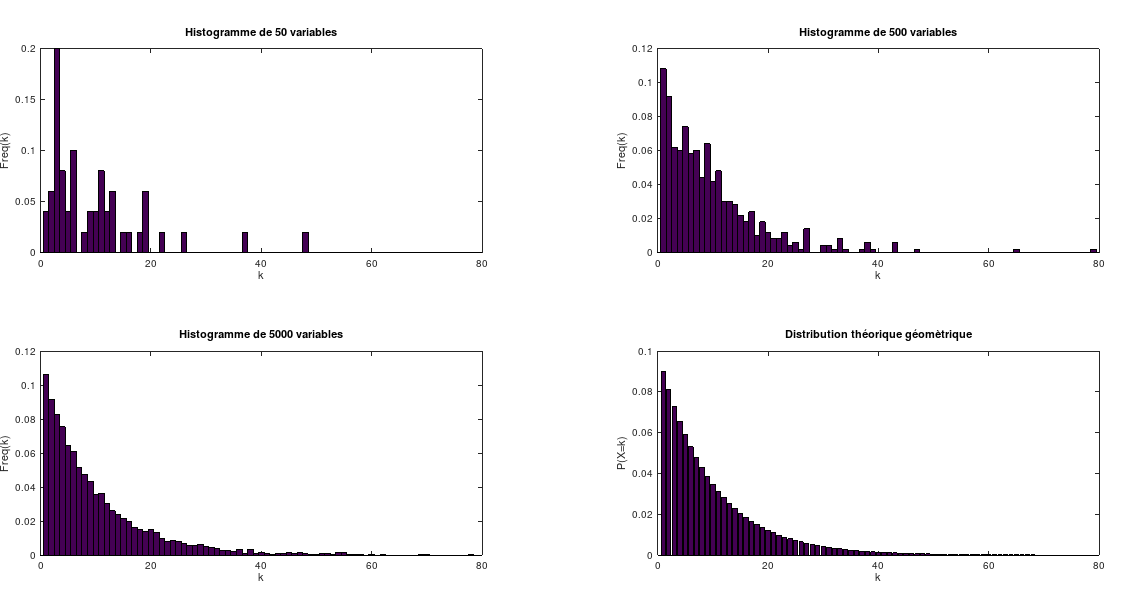
\includegraphics[scale=0.3]{images/histGeom.png} 
\end{center}
 \caption{Histogrammes et distribution de loi géométrique}
 \label{Histogrammes et distribution de loi géométrique}
\end{figure}

On observe bien que les histogrammes se rapprochent de la distribution théorique quand
la taille de l'échantillon est grande (plusieurs milliers).

Pour générer les populations , on utilise la fonction "geomGen" qui simule
n expériences où, pour chacune d'entre elle, on effectue un enchainement
d'épreuve de Bernouilli en générant une variable de loi uniforme sur
$[0;1]$ . Si la valeur obtenu est supérieure à p, on arrête la boucle
et la valeur générée est égale au nombre d'épreuves, sinon on continue 
jusqu'à obtenir cette condition. Le code Matlab (Octave) utilisé est :

\lstinputlisting[language=Matlab]{src/geomGen.m}


\subsection{Estimateurs du maximum de vraisemblance}

L'estimateur $\hat{p}$ du maximum de vraisemblance est la valeur qui
maximise la loi de vraisemblance L(p) : $\hat{p}=argmax(L(p))$.
On calcule L(p) dans un premier temps :
\[L(p)=L(X_1(p),X_2(p),...,X_n(p))=\prod\limits_{i=1}^{n}(1-p)^{X_i-1}p 
\]
avec $X_i,\ i\in\{1,..,n\}$ les variables d'échantillon.
\[L(p)=p^n(1-p)^{(\sum\limits_{i=1}^{n}X_i)-n}\]
On peut effectuer un passage au logarithme pour trouver un maximum car il s'agit
d'une fonction strictement croissante (et défini sur $]0;1]$). L'argument du maximum du logarithme
de $L(p)$ et du maximum de $L(p)$ sont les mêmes.
\[\log{L(p)}=n\log{p}+((\sum\limits_{i=1}^{n}X_i)-n)\log{(1-p)}\]
\[\frac{d\log{L(p)}}{dp}=\frac{n}{p}-\frac{(\sum\limits_{i=1}^{n}X_i)-n}{1-p}\]
\[\text{On a }\frac{d\log{L(\hat{p})}}{dp}=0\]
\[\text{Donc }\frac{n-n\hat{p}-((\sum\limits_{i=1}^{n}X_i)-n)\hat{p}}{\hat{p}(1-\hat{p})}=0\]
\[\text{Ce qui implique (dans le cas différent de 0 et 1) }n-(\sum\limits_{i=1}^{n}X_i)\hat{p}=0\]
Finalement :
\[\hat{p} = \frac{n}{\sum\limits_{i=1}^{n}X_i}\]

Si la résolution analytique pour trouver l'estimateur avait été impossible,
l'utilisation d'un algorithme d'optimisation (comme une descente de gradient) ou encore
l'utilisation d'une fonction d'intégration aurait été possible.

\subsection{Test de l'estimateur}

Afin de tester l'estimateur du maximum de vraisemblance pour différent taille
d'échantillon, on utilise le code suivant :

\lstinputlisting[language=Matlab]{src/deltaEspEstGeom.m}

\begin{figure}[!h]
\begin{center}
 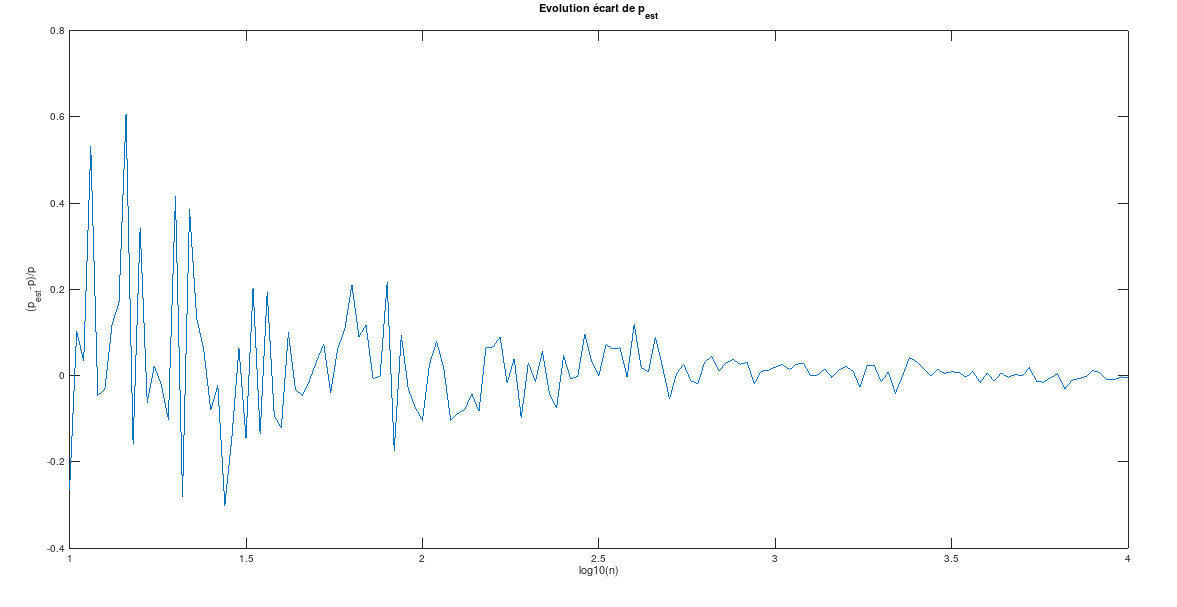
\includegraphics[scale=0.3]{images/biaisGeom.png} 
\end{center}
 \caption{Evolution du biais de l'estimateur}
 \label{Evolution du biais de l'estimateur geom}
\end{figure}

On voit que

On effectue la ...

\lstinputlisting[language=Matlab]{src/deltaEstGeom.m}

\begin{figure}[!h]
\begin{center}
 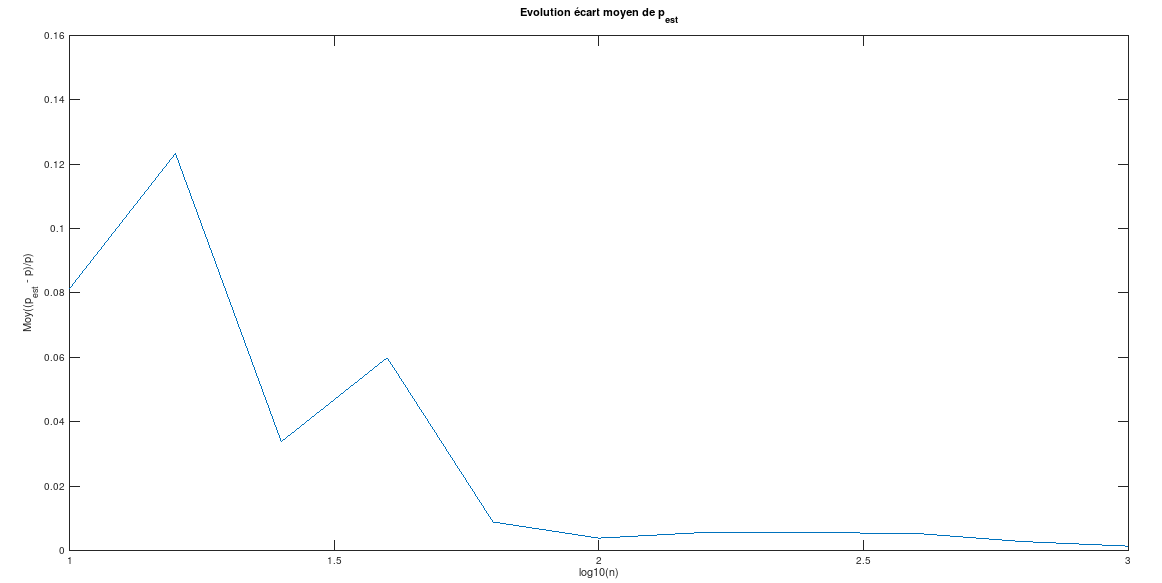
\includegraphics[scale=0.3]{images/biaisMoyGeom.png} 
\end{center}
 \caption{Evolution du biais moyen de l'estimateur}
 \label{Evolution du biais moyen de l'estimateur geom}
\end{figure}

\subsection{Loi extrême}



\section{Loi de Cauchy}
\end{document}


